\section{Application expérimentale}
\label{sec:app}

\epigraph{Le monde est tout ce qui a lieu.}{Ludwig Wittgenstein\\\textsc{Tractacus
    Logico-Philosophicus}}

Pour conclure ce mémoire, nous offrons au lecteur une brève application de la méthode
algorithmique présentée à la Section \ref{sec:kernel}. Le but ici n'est pas nécessairement
d'offrir une intuition sur le comportement fondamental des marchés, mais plutôt
d'illustrer de quelle façon un technicien pourrait mettre en œuvre un algorithme
d'investissement en utilisant une approche d'apprentissage machine régularisée simple.

Le cadre expérimental sera le suivant: le rendement aléatoire $R$ sera celui du titre AMZN
et les variables de marché $X_j$ seront obtenues à partir de la valeur à la fermeture des
marchés des indices NASDAQ et VVIX (voir Figure \ref{fig_corr1}). Ces valeurs seront
obtenues à partir du 1\ier janvier 2004 jusqu'au 15 août 2017, ce qui représente un
échantillon de 3429 points. Ces données brutes seront d'abord normalisées sur toute la
période considérée puis transformées en considérant les moyennes et les écarts type de ces
variables lors des cinq jours précédants de façon à avoir dix variables de marché
(incluant le biais). La Table \ref{table_corr} précise la nature de chacune de ces
variables.

\begin{figure}[h]
  \centering
  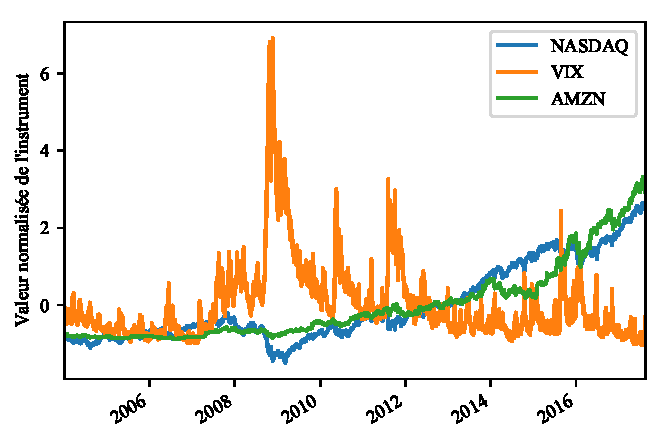
\includegraphics[width=\textwidth]{../experiments/fig/corr1.pdf}
  \caption[Evolution des variables de marché]{Evolution temporelle de valeur à la
    fermeture du titre AMZN et des indices VIX et NASDAQ sur un échelle commune.}
  \label{fig_corr1}
\end{figure}

\begin{table}[h]
  \centering
\begin{tabular}{ll}
  \toprule
  Variable  & Signification\\
  \midrule
  $R$ & Rendement d'AMZN à $t+1$\\
  $X_0$ & Terme de biais constant à 1\\
  $X_1$ & Rendement normalisé du NASDAQ à $t$\\
  $X_2$ & Rendement normalisé du VIX à $t$\\
  $X_3$ & Rendement normalisé d'AMZN à $t$\\
  $X_4$ & Moyenne de $R$ sur $[t-5,t]$\\
  $X_5$ & Moyenne de $X_1$ sur $[t-5,t]$\\
  $X_6$ & Moyenne de $X_2$ sur $[t-5,t]$\\
  $X_7$ & Ecart type de $R$ sur $[t-5,t]$\\
  $X_8$ & Ecart type de $X_1$ sur $[t-5,t]$\\
  $X_9$ & Ecart type de $X_2$ sur $t[t-5,t]$\\
  \bottomrule
\end{tabular}
\caption{Variables de marché employée dans le cadre de cette expérience.}
\label{table_corr}
\end{table}

En second lieu, la fonction d'utilité employée au cours de cette expérience sera de type
Lipschitz exponentielle (voir Section \ref{sec:emp}) avec paramètre d'échelle $\mu = 3$. La
Figure \ref{fig_corr2} présente cette fonction d'utilité par rapport à la distribution des
rendements normalisés d'AMZN ainsi que la distribution $u(R)$ de l'utilité appliquée à ce
rendement aléatoire. On obtient alors une utilité moyenne (obtenue sans décision)
$\hE u(R)=\num{-0.0657}$. Par ailleurs, pour des raisons computationnelles, nous nous
limiterons à un noyau linéaire. Notons que le choix de ces paramètres est tout à fait
arbitraire, mais souhaite représenter le type d'utilité dont un véritable investisseur
pourrait souhaiter se voir doter.

\begin{figure}
  \centering
  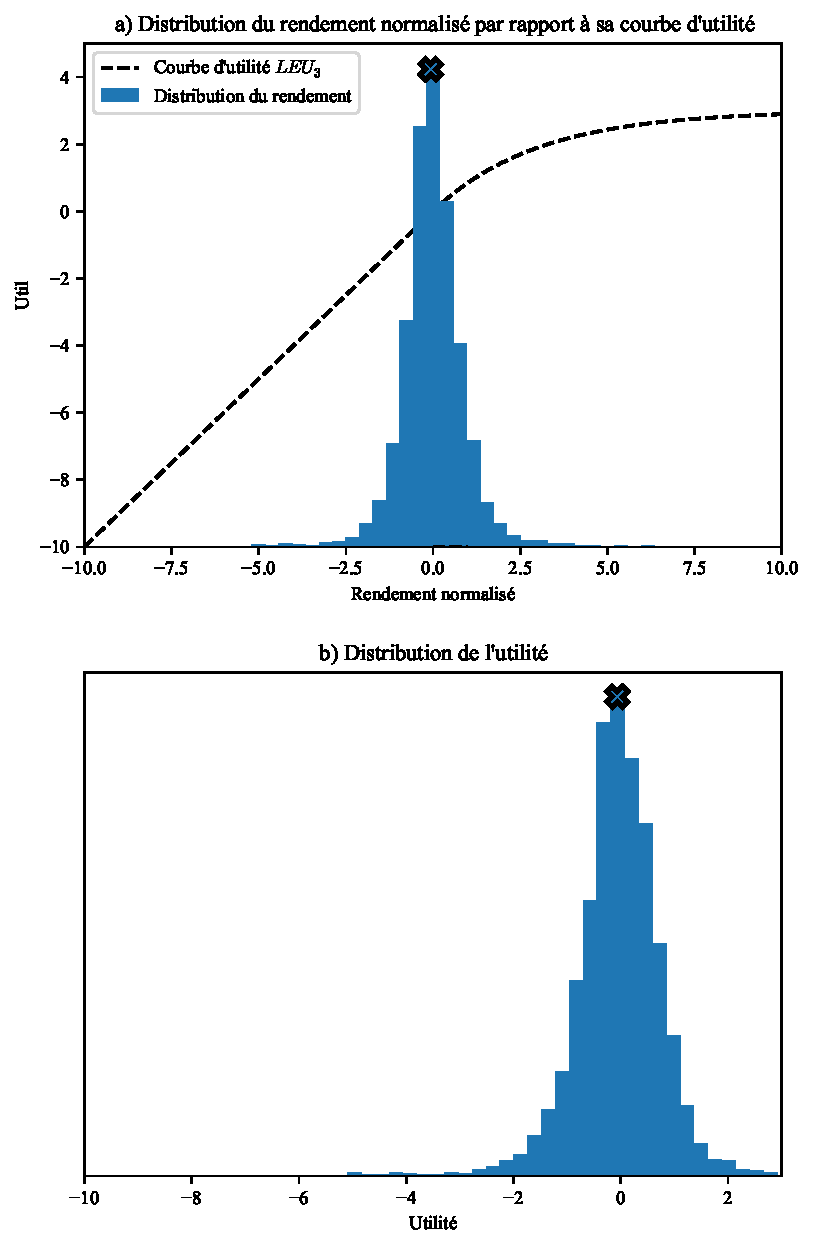
\includegraphics[width=0.9\textwidth]{../experiments/fig/corr2.pdf}
  \caption[Distribution des rendements et de l'utilité]{Le panneau a) présente la
    distribution des rendements de AMZN du 1\ier janvier 2004 jusqu'au 15 août 2017 ainsi
    que le comportement de la fonction d'utilité $\LEU_3$ sur un domaine commun. Le
    panneau b) illustre l'effet de la fonction d'utilité sur ces rendements. Les deux
    croix indiquent où se situent les moyennes empiriques de ces deux distributions. On a
    respectivement $\hE(R) = \num{0.000409}$ et $\hE u(R) = \num{-0.0657}$.}
  \label{fig_corr2}
\end{figure}

L'ensemble de test sera composé des 686 derniers jours, soit du 1\ier décembre 2014
jusqu'au 15 août 2017. L'ensemble d'entraînement sera formé des 2740 jours restants. Pour
déterminer le facteur de régularisation à employer, on procèdera par validation
croisée. Cette méthode consiste d'abord à scinder l'ensemble d'entraînement en plusieurs
groupes de même taille (cinq dans ce cas-ci). Puis, tour à tour, chaque groupe joue le
rôle de l'ensemble de validation alors que les autres groupes constituent l'ensemble
d'entraînement. Ceci permet d'optimiser la performance moyenne atteinte sur les
échantillons de validation en modifiant le paramètre de régularisation $\lambda$. Par exemple,
la Figure \ref{fig_corr3} indique les différentes valeurs d'utilité moyenne en
entraînement et en validation selon $\lambda$. On peut ainsi optimiser le paramètre de
régularisation sans jamais n'avoir recours à l'ensemble de test. Ceci permet alors de
trouver un paramètre de régularisation optimal $\lambda = \num{0.001}$.


\begin{figure}
  \centering
  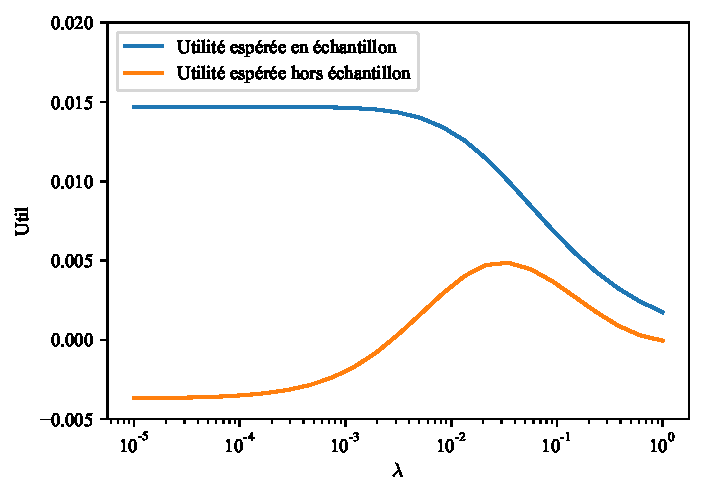
\includegraphics[width=\textwidth]{../experiments/fig/corr3.pdf}
  \caption[Optimisation de $\lambda$]{Figure d'optimisation de paramètre de régularisation. En
    fixant l'ensemble d'entraînement et de validation, on fait varier $\lambda$ sur une échelle
    logarithmique afin de déterminer la meilleure régularisation à appliquer.}
  \label{fig_corr3}
\end{figure}


À partir de cette valeur, on est alors en mesure de déterminer une fonction
d'investissement $\qh$ optimale puis de calculer à partir des ensembles d'entraînement et
de test l'utilité moyenne atteinte sur l'échantillon d'entraînement et sur l'échantillon
de test. On finit par obtenir une utilité moyenne en entraînement de \num{0.013487} et de
\num{0.005354} sur l'ensemble de test. Les composantes de la fonction de décision $\qh$
ainsi obtenue sont données à la Table \ref{table_q}.  


\begin{table}[h]
  \centering
\begin{tabular}{lr}
  \toprule
  Variable  &  $\qh$\\
  \midrule
  $X_0$ & \num{0.237228 }\\
  $X_1$ & \num{-0.180824}\\
  $X_2$ & \num{-0.004759}\\
  $X_3$ & \num{0.219300 }\\
  $X_4$ & \num{-0.227734}\\
  $X_5$ & \num{-0.116276}\\
  $X_6$ & \num{0.061316 }\\
  $X_7$ & \num{-0.447030}\\
  $X_8$ & \num{0.205306 }\\
  $X_9$ & \num{-0.116650}\\
  \bottomrule
\end{tabular}
\caption{Composantes de $\qh$ pour chacune des variables de marché.}
\label{table_q}
\end{table}

Ces résultats sont donc assez encourageants puisqu'en comparaison, un investisseur dont
l'unique action serait de détenir le titre, \ie\ d'appliquer une fonction de décision
$q_0(x) = 1$ pour toute réalisation $x$ obtiendrait une utilité espérée sur le même
ensemble de test de $\hEU(q_0) = \num{-0.0175}$. De plus, un investisseur qui baserait sa
décision que sur le rendement en entraînement, \ie\ où $\qh$ ne serait déterminé qu'avec
la variable de marché de biais obtiendrait alors une décision constante
$q_1(x) = \num{-0.0305}$, ce qui lui fournirait une utilité moyenne hors échantillon de
\num{-1.25e-5}.



% Cependant, les résultats ainsi obtenus dépendent alors fortement des ensembles
% d'entraînement et de test, tel qu'illustré à la Figure \ref{fig_corr4}. En substance, on
% obtient alors une utilité espérée en échantillon moyenne (sur un échantillon de 500
% points) de \num{0.014164} alors que l'utilité espérée hors échantillon moyenne est de
% \num{-0.001349}. Bien que l'utilité hors échantillon moyenne soit légèrement négative, il
% n'en demeure pas moins que notre technique permet d'améliorer sensiblement l'utilité
% espérée moyenne $\hE u(R)$.

% Par ailleurs, la Figure \ref{fig_corr4} semble indiquer que l'hypothèse centrale sur
% laquelle repose ce mémoire, \ie\ le caractère \iid\ de la loi de marché $M$ n'est peut
% être pas respectée! En effet, si $M$ était vraiment \iid, on s'attendrait à ce que les
% performances en échantillon et hors échantillon ne dépendent pas autant de
% l'échantillonage employé. Mais il est également possible que l'échantillonage soit trop
% faible, ce qui ne permettrait alors pas de réduire suffisament l'incertitude.

Il est important de comprendre que la qualité des résultats sera nécessairement limitée
par les variables $X_j$ utilisées. Pour faire un travail appliqué plus complet, il serait
nécessaire d'avoir d'abord une bonne intuition et une bonne expérience des facteurs
fondamentaux qui viennent affecter les mouvements de marché. Ceci dépasse cependant le
cadre de ce travail, qui se veut avant tout intéressant sur le plan théorique et
méthodologique.

De plus, il pourrait être intéressant de considérer d'autres fonctions d'utilité. En
effet, une utilité $\LEU_\mu$ est peut être trop agressive puisqu'elle est bornée par
$\mu$. Au contraire, une utilité log Lipschitz (linéaire sur les rendements négatifs et de
progression logarithmique sur sa branche de droite) ne serait pas bornée et pourrait donc
possiblement offrir des résultats plus intéressants.

Par ailleurs, ces résultats n'ont été obtenus qu'à partir d'un noyau linéaire. Un travail
plus complet examinerait la différence de performance obtenue avec d'autres types de
noyaux.

Il est par ailleurs fort possible qu'avec une meilleure intuition financière permettant de
choisir de meilleures variables et en employant un noyau plus général (par exemple
gaussien), un investisseur pourrait réellement déterminer une fonction de décision
efficace lui permettant d'obtenir une utilité moyenne élevée.

En conclusion, cette expérience a permis de montrer comment on pouvait obtenir des
résultats intéressants en n'utilisant que quelques variables de marché. Rappelons que
l'avantage qu'apporte l'algorithme d'investissement décrit dans ce mémoire est d'optimiser
directement l'effet que peuvent avoir les variables de marché sur l'utilité espérée, et
non pas de simplement chercher à obtenir une régression sur les rendements à partir de ces
variables, comme on pourrait être tenté de le faire. On pondère ainsi chacune des
variables non pas par sa relation avec le rendement, mais plutôt la façon dont elles
parviennent à procurer à un investisseur une utilité moyenne plus grande.

% \begin{figure}
%   \centering
%   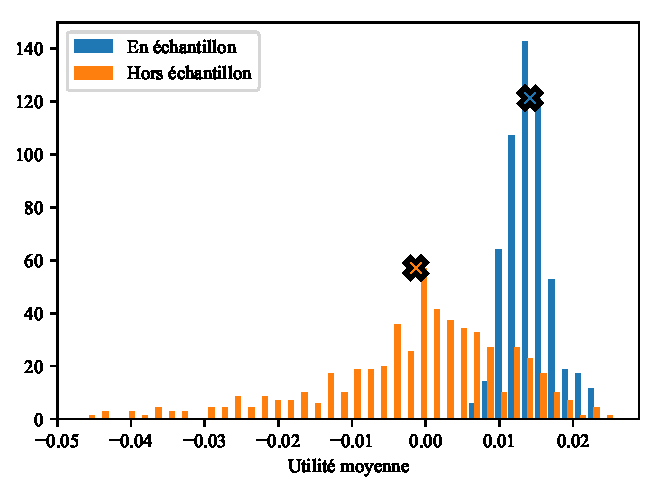
\includegraphics[width=\textwidth]{../experiments/fig/corr4.pdf}
%   \caption[Distribution de l'utilité espérée en et hors échantillon]{Distribution de
%     l'utilité espérée en échantillon et hors échantillon avec paramètre de régularisation
%     constant à $\lambda = \num{7.262e-3}$. Plus précisément, un ensemble d'entraînement
%     aléatoire formé de quatre cinquièmes des données et d'abord formé, duquel on détermine
%     une fonction d'investissement $q$. L'utilité moyenne hors échantillon est ensuite
%     calculé sur le cinquième des données restantes. Les deux croix indiquent la moyenne
%     des utilité espérées en et hors échantillon, respectivement de \num{0.014164} et de
%     \num{-0.001349}.}.
%   \label{fig_corr4}
% \end{figure}


%

% La question de l'hypothèse du marché $M$ comme une loi \iid\ se pose ici à nouveau. En
% effet, si cette hypothèse était véritablement respectée, le choix de l'ensemble de test ne
% poserait aucun problème puisqu'ils seraient alors tous équivalents. Néanmoins, puisqu'on
% est en présence d'un processus foncièrement temporel, il devient tentant de prendre comme
% ensemble de test les derniers 


\clearpage




%%% Local Variables:
%%% mode: latex
%%% TeX-master: "memoire"
%%% End:
